\documentclass[12pt, a4paper]{article}

\usepackage{cmap}
\usepackage[utf8]{inputenc}
\usepackage[T1]{fontenc} 
\usepackage[british]{babel}
\usepackage{hyperref}
\usepackage{listings}
\usepackage{xcolor}
\usepackage{booktabs}
\usepackage{amsmath,amssymb}
\usepackage{tikz}
\usepackage{verbatim}
\usepackage{datetime}

\sloppy
\newdate{current_change_date}{02}{05}{2026}
\date{\displaydate{current_change_date}}

\usetikzlibrary{positioning}


\definecolor{codegreen}{rgb}{0,0.6,0}
\definecolor{codegray}{rgb}{0.5,0.5,0.5}
\definecolor{codepurple}{rgb}{0.58,0,0.82}
\definecolor{backcolour}{rgb}{0.95,0.95,0.92}

\lstset { %
    language=C++,
    backgroundcolor=\color{black!5}, % set backgroundcolor
    basicstyle=\ttfamily,% basic font setting
    captionpos=b, 
    commentstyle=\color{codegreen},
    keywordstyle=\color{blue},
}

\title{Listening, Speaking, Thinking}
\author{Tatyana Chistyakova}

\begin{document}
\maketitle
\begin{abstract}
The article presents a conceptual framework for constructing a model of the human brain. 
The outcome is a program that demonstrates the ideas outlined in the paper. The study 
does not aim at the practical application of the program; rather, its 
primary objective is to investigate the theoretical feasibility of developing such a system. 
\end{abstract}
\section{Philosophical concepts}


This chapter outlines the foundational philosophical concepts that served as starting 
points for the present work. These concepts are expressed in an informal 
manner and are not treated as strict laws; rather, they are regarded as 
guiding ideas and intuitions underpinning the formal developments presented in subsequent chapters.

Aristotle’s doctrine of categories and syllogisms introduces the notions 
of generality and particularity, thereby illustrating the organisation of 
knowledge and memory in a hierarchical structure.

George Boole’s theory of thought\cite{Boole} (distinct from Boolean algebra) provides 
a framework for operations on knowledge, such as AND and XOR. In addition, 
human cognition employs predicate logic, quantifiers, and higher-order logical systems.

The axiomatic framework of set theory\cite{Zermelo–Fraenkel_set_theory} 
may be interpreted, under the assumption that mathematics constitutes a science of 
human thought, as describing the most primitive elements of cognition. These 
elements can be identified as sets and functions defined over them.

The structure of the neuron is also considered. Contemporary artificial 
neural networks fall outside the scope of this work; the focus here is 
on the biological neuron. A neuron can exist in two distinct states 
depending on the incoming potential, suggesting that the human brain 
may possess a fundamentally digital rather than analogue nature. This 
observation aligns with Boole’s proposal of two basic states, TRUE and FALSE, 
as the foundational units of knowledge.

The fundamental components required for sentence construction are nouns, 
adjectives, and verbs\cite{Part_of_speech}. Nouns and verbs are present in all known 
languages, whereas adjectives may, in certain cases, be replaced 
by adverbs.

The distinction between P and NP complexity classes remains unresolved; 
however, it is widely conjectured that they are not equal. This 
work proceeds under the assumption that $P \ne NP$. This assumption 
is significant because any algorithm executable on a conventional 
computer is constrained to P-complexity, whereas humans routinely 
solve problems of apparent NP-complexity. Consequently, the 
underlying computational model must correspond to a non-deterministic 
Turing machine.

Extrapolation is another essential cognitive ability. Even young children 
demonstrate the capacity to extrapolate from limited data, indicating 
that this ability is, at least in part, innate and further developed over time. 
In most practical contexts, extrapolation constitutes an NP-complex problem. 
Moreover, such problems typically admit multiple valid solutions, implying that 
humans are capable of generating and selecting among several possible answers.

In addition to handling NP-complexity\cite{P_versus_NP_problem}, a critical 
feature of human cognition is the apparent inability to enter an infinite loop. 
Any Turing-complete system may become trapped in a non-terminating computation, 
whereas humans maintain control over their cognitive processes. This suggests 
that human information processing may be more accurately modelled by a finite 
automaton without unbounded cycles.

A related constraint applies to logic itself. G\"odel’s second incompleteness theorem 
asserts that a system cannot prove its own consistency, as doing so would entail a 
form of logical circularity. Notably, this result is formulated within the language 
of Boolean algebra. Therefore, although humans can intuitively grasp such logical 
systems, they cannot employ them in a fully unrestricted manner.

To account for this limitation, the present work draws upon socionics\cite{Socionics} 
-- a non-academic framework positing the existence of sixteen cognitive types defined 
by four dichotomies. The interpretation of socionics used here is original and may not align with other 
formulations. Its inclusion is motivated by the observation that classical academic 
theories often assume unconstrained cognition, thereby conflicting with G\"odel’s theorem.


\section{Mathematical representation}

\lstMakeShortInline|

From here on the code from the following repository is used. 

\begin{center}
  \url{https://github.com/TaniaChistyakova/brain.git}
\end{center}


The operations AND and XOR defined on the set $\{0, 1\}$ form monoids, as each possesses 
an identity element and satisfies associativity. Moreover, XOR admits an inverse 
operation, namely 1 XOR X. Consequently, taken together, these operations define a ring 
over this set. Since AND is also commutative, the resulting structure is a commutative 
ring. In the implementation, the AND operation corresponds to the operator |&|, while 
XOR corresponds to |^|. The elements of the binary set are represented by the class |Dot|. 
In the mathematical exposition, AND is denoted by $\land$ and XOR by $\oplus$.

The codebase includes several classes for representing binary sequences. The 
class |DotArray| describes binary sequences of arbitrary length, whereas |DotFixedArray| 
represents sequences of fixed, predefined length.

Using AND and XOR, any function $f:*\{0,1\}\to*\{0,1\}$ mapping binary inputs to binary 
outputs with an arbitrary number of arguments can be expressed in algebraic normal 
form. This representation is advantageous because it is unique, computationally 
efficient, and admits straightforward definitions of AND and XOR operations. In 
the implementation, such functions are encapsulated by the class VectorFunction.

Hereafter, the terms ``function'' or ``vector function'' refer to functions defined 
over the space of binary sequences with an arbitrary number of arguments, 
represented in algebraic normal form. A similar function that returns a value 
in $\{0, 1\}$ will be referred to as a scalar function. It is important to note 
that a function occupies a specific amount of memory: if it accepts $n$ arguments 
and produces $m$ outputs, it requires $(m * 2^n)$ bits of storage.

Any subset of a finite-dimensional binary sequence space can be specified via a 
projection operator (projector). For such projectors, AND and XOR operations can 
likewise be defined, corresponding to the respective operations on the 
sets they represent. In the code, this abstraction is implemented as the class |Projector|.

One may then define scalar binary functions over spaces of projectors or 
binary functions. Such higher-level mappings will be referred to as functors. 
A functor can be used to define a wide range of universal syntactic constructions. 
In order to specify a scalar function of $k$ arguments unambiguously, $2^k$ bits 
are required. Accordingly, if one employs unary operations (such as NOT), binary 
operations (such as OR and $\to$)\cite{Material_conditional}, and ternary operations (such as 
|x = a ? b : c|)\cite{Ternary_conditional_operator}, their complete specification 
requires only 8 bits. In the implementation, this concept corresponds to the class |Functor|.

Finally, projectors and functions are combined into elementary finite automata referred to as 
``sentences''. These automata scan continuous streams of binary data in search of specific 
sequences interpreted as nouns. Upon detection, they identify a finite set of subsequences 
interpreted as adjectives, and the results of this detection are then supplied as inputs 
to a function. This mechanism is implemented in the class |Sentence|.



\begin{lstlisting}[caption=Sentence in pseucode]
class Sentence: public ContextObject
{
public:
  //.................

  Projector const *                 noun;
  VectorFunction const *            verb;
  std::vector<const Projector *>    adjectives;
};
\end{lstlisting}


In order to realise higher-order logic, it is necessary that all of the constructs described 
above--projectors, functions, and sentences--serve not only as operational entities but also 
as data objects for themselves. In other words, higher-order projectors must operate over 
a generalised space comprising functions and projectors of lower order. This is achieved 
by assigning to each object a unique code represented as binary data accessible for 
processing. The computation of such a code is performed by the class |HashCalculator| 
and is based on the intrinsic structure of each object. An important advantage of this 
approach is that it allows all object codes to be constructed with a uniform size.

The class |HashCalculator| thus transforms an object into data, while the inverse transformation 
-- from data to object -- is carried out by another class, |Context|. The context not only 
performs the function of reconstructing objects from data, but also serves as a quantifier 
over lower-order objects. Consequently, in order to regulate the order of logic, contexts 
must be organised into a well-defined hierarchy, within which the highest-level context is 
referred to as the global context.

Since projectors, functions, and sentences acquire a shared functionality for handling 
such codes, a common base class, |ContextObject|, is introduced.


\begin{lstlisting}[caption=Context]
class Context
{
public:
  // initialises the current context, 
  // if no parent the current context is global
  Context(const Context* inParent);

  const Context* GetParent() const;

  // adds a new object into the current context
  // ContextObject is the base class 
  // for functions, projectors and sentences
  Word AddNew(const ContextObject* pObj);

  // there is no remove operation 
  // for a context object, 
  // all the objects should be destroyed 
  // in the context

  // searches for a object 
  // through all the context's hierarchy
  ContextObject const* Get(Word code) const;

};
\end{lstlisting}

The use of |HashCalculator| necessitates the specification of a code length representing 
each object. This length, however, directly determines the number of distinct ``words'' 
available within the mental lexicon of a human. Consequently, it cannot be chosen to 
be either excessively large or excessively small. Empirical studies suggest that the 
average human vocabulary comprises approximately 10–12 thousand word 
families\cite{Brysbaert2016-om}. This implies that a 14-bit identifier is sufficient 
to encode each word uniquely. In the implementation, this is realised by the class 
|Word|, which is defined as |DotFixedArray<14>|.

Nevertheless, natural language is not limited to words alone. It also requires conjunctions, 
which are here modelled using functors, and punctuation marks, which serve to denote 
sentences. In order to distinguish between these three fundamental categories, along 
with a fourth null category, an additional 2 bits are required. As a result, the minimal 
unit of the language has a total length of 16 bits and is denoted as |Letter|. For practical 
reasons, |Letter| is implemented as |uint16_t| rather than as |DotFixedArray<16>|. 
The complete logic governing the decoding of linguistic symbols is described in detail 
in the file Letter.h and is summarised in Table \ref{tab:symbols}.

\lstDeleteShortInline|

\begin{table}
\begin{center}
\begin{tabular}{ | l | l | l | } 
 \toprule
 Part of Speech  & C++ type             & Size in bits      \\ 
 \midrule
 any object      & \lstinline!Letter!   & 16                \\ 
 word            & \lstinline!Word!     & 14                \\ 
 conjunction     & \lstinline!Functor!  & $\leqslant 8+2$   \\ 
 punctuation     & \lstinline!Sentence! & 5                 \\ 
 \bottomrule
\end{tabular}
\end{center}
\caption{All language symbols}
\label{tab:symbols} 
\end{table}

\lstMakeShortInline|

It is necessary to justify the chosen parameter sizes. As noted previously, 8 bits of data 
are sufficient to describe a ternary operator using a functor. In addition, 2 further 
bits are required to distinguish between unary, binary, and ternary operators. This 
accounts for the expression 8+2 in the case of conjunctions.

Punctuation is represented in the form of a sentence. A sentence contains two fixed 
components--a noun and a verb--and a variable number of adjectives. It is precisely this 
number that determines the size of the sentence. While the sizes of words and conjunctions 
admit relatively straightforward justification, no equally rigorous rationale is available 
for the size of a sentence. Nevertheless, a 5-bit allocation was chosen, allowing for up 
to $13 \times 2$ adjectives.

This value may appear relatively large and potentially unrealistic. However, it was motivated 
by considerations of how arithmetic might be represented within the proposed sentence 
framework. Most practical numeral systems employ 10 digits, while historical systems have 
used up to 12. Attempts to introduce systems with a larger number of digits have generally 
proven impractical for mental computation and have effectively decomposed into multiple subsystems.

Within this framework, a basic sentence may take the form of a noun such as ``is this a 
digit?'', accompanied by a set of adjectives such as ``is this zero?'', ``is this one?'', 
and so forth up to nine. Additionally, it is necessary to determine the positional 
value of the digit, for example, ``is this units?'', ``is this tens?'', or ``is this hundreds?''. 
This results in a total of 13 adjectives when employing a decimal system with three positional 
groupings. In this manner, both the value of each digit and its positional role can be 
determined in a single operation. Notably, the resulting structure bears a strong 
resemblance to the Ancient Greek numeral system\cite{Greek_numerals}.

However, a human being is capable not only of mental counting but also of performing 
arithmetic operations. To carry out a single operation, thirteen adjectives are no 
longer sufficient; it becomes necessary to construct an operation involving two 
digits. Each digit, in turn, requires a complete description. Consequently, this 
yields $13 \times 2$ adjectives.

From a lexical perspective, a punctuation mark may be interpreted as a sequence of commas 
of variable length, terminated by a full stop.

Empirical observations suggest that other mammals are also capable of distinguishing 
multiple qualitative features in incoming data. For example, dogs can recognise several 
distinct quantities--typically up to three or four--rather than merely ``one'' and 
``many''\cite{psychologytodayDogsKnow}. This may indicate that, in such systems, 
punctuation-like structures are effectively represented using 2 bits.

To enable the use of letters, a specialised container referred to as a ``layer'' 
is introduced. This structure is implemented as a queue with a fixed maximum capacity, 
thereby preventing overload. New symbols are added to the front, while older symbols 
are automatically removed from the rear. The indexing mechanism inherently accounts for 
the removal of outdated elements. In the implementation, this structure corresponds to the 
class |Layer|. Although functions and projectors operate with bit-level access, interaction 
with the layer is aligned to the size of a letter. This alignment is necessary to ensure 
the correct handling of auxiliary symbols associated with each individual letter.

\section{Operation of Objects}

\paragraph{Structure of the Information Space}

The operation of objects is defined within an abstract, conditionally three-dimensional 
space. This space is not Euclidean in the conventional sense; however, each object is 
associated with a set of coordinates. Of the three axes, two are of primary importance: 
the vertical and the horizontal. The third axis, representing depth, is present only 
implicitly, without explicit references or numerical coordinates. This construct 
will be referred to as the information space, and each point within it is assigned 
coordinates of the form $[n,m]$, where $n$ and $m$ are natural numbers. The first component 
denotes the vertical coordinate, while the second denotes the horizontal coordinate.

At each point in the information space, there exists exactly one layer. It should be 
emphasised, however, that due to the three-dimensional nature of the space, each pair 
of planar coordinates corresponds to a set of points distinguished by depth, and each 
such point possesses its own distinct layer.

\begin{figure}[h]
\begin{center}
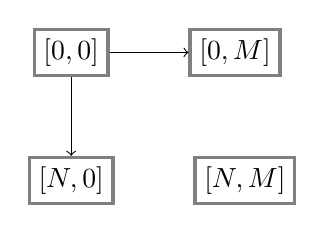
\begin{tikzpicture}[
squarednode/.style={rectangle, draw=black!50, very thick, minimum size=5mm},
]
%Nodes
\node[squarednode]      (upleft)                            {$[0, 0]$};
\node[squarednode]      (downleft)      [below=of upleft]   {$[N, 0]$};
\node[squarednode]      (upright)       [right=of upleft]   {$[0, M]$};
\node[squarednode]      (downright)     [below=of upright, right=of downleft] {$[N, M]$};

%Lines
\draw[->] (upleft.south) -- (downleft.north);
\draw[->] (upleft.east) -- (upright.west);
\end{tikzpicture}
\end{center}
\label{fig:infospace}
\caption{Coordinates in the informational space}
\end{figure}

The point with coordinates $[0,0]$ is located in the upper-left corner; there exist no 
points either above or to the left of it. The lower-left boundary is given by the 
coordinate $[N,0]$, where $N$ denotes the maximum number of layers. The upper-right 
boundary is defined by $[0,M]$, where $M$ is a predetermined maximum horizontal 
rank of the response tree. These coordinates collectively determine the limits of 
the information space.

Within this system, information propagates initially in the upward vertical direction, 
then horizontally to the right, and subsequently downward. The dimensions of this space 
are finite, ensuring that information does not escape its bounds. The circulation of 
information is governed by the class |Neocortex|, which, upon instantiation, is 
provided with the numerical limits of the internal information space.

\paragraph{Initialisation of Long-Term Memory and Construction of Input Layers}

Prior to the operation of the neocortex and its associated information space, the 
input layers are initialised and long-term memory is loaded. It is assumed that an 
appropriate number of layers is six\cite{Neocortex}. Long-term memory is placed at 
the node $[0,0]$, at the topmost position across all layers.

It is important to state a key assumption regarding long-term memory. Within this 
model, long-term memory is static and does not change. In practice, this is not 
the case: long-term memory is continuously updated, both through the acquisition of new 
knowledge and the loss of outdated information.

In the present framework, however, this loading occurs only once at the initial stage, 
when short-term memory is still empty. During subsequent stages, short-term memory 
begins to accumulate, and the model no longer permits modification of long-term memory, 
since short-term memory is largely derived from it. Only those patterns that can be 
expressed in terms of long-term memory are detectable; any information not predefined 
within it is effectively ignored.

In the implementation, this procedure is carried out by the method 
|Neocortex::SetGlobalContext()|.

\paragraph{Acquisition of Input Data and Projectors over Input Layers}

The initial input information is represented as an array of words, 
|std::deque<Word>|, and is transformed into an array of letters by appending two 
additional bits to each word, indicating its classification as a word. This array of 
letters is then placed at the input point of the information space with coordinates 
$[N,0]$. This procedure is implemented in the method |Neocortex::SetInput()|.

In contrast to the loading of long-term memory, which occurs only once, the input 
of data is a recurring process. It is executed within the main operational loop 
and initiates each new iteration of processing. The data contained in the word array 
may correspond both to external sensory inputs -- such as auditory signals, visual patterns, 
and tactile sensations -- and to internal states, including levels of arousal or emotional 
conditions. Within the framework of Robert Plutchik’s wheel of 
emotions\cite{Emotion_classification}, emotional states can be represented as points in a 
two-dimensional Euclidean space. Accordingly, each input includes two words dedicated 
to the representation of emotional state.

Immediately following the acquisition of new input, a recognition process is initiated. 
The global context sequentially evaluates all of its projectors for matches; when a 
match occurs and the corresponding projector has not been previously activated, 
its associated word is propagated to the next layer. Consequently, if a sequence 
contains multiple consecutive words of the same type recognised by a single projector, 
the corresponding word is transmitted to the higher layer only once. This mechanism 
enables the extraction of meta-information from symbol sequences of arbitrary length.

The input signal itself may be arbitrarily long, potentially comprising thousands 
of symbols of the same type and even extending across multiple input instances. 
Nevertheless, it remains subject to correct recognition. This reflects a fundamental 
property of humans and other mammals: the ability to process and recognise effectively 
unbounded sequences of signals, as well as to generate correspondingly unbounded responses.


\begin{figure}[h]
\begin{center}
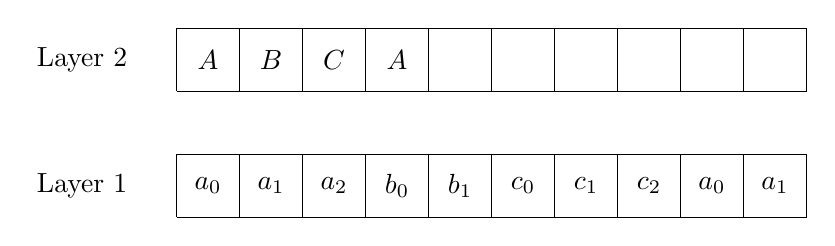
\begin{tikzpicture}[scale=0.4]


\def\y{0}
\node at (-3+2*0,1+\y) {Layer 1};
\draw (0,2+\y) -- (20,2+\y);

    \def\xa{0}
    \foreach [evaluate=\xa as \x using {int(\xa+\xb)}] \xb in {0,...,2}
    {
        \draw (0+2*\x,0+\y) -- (0+2*\x,2+\y);
        \node at (1+2*\x,1+\y) {$a_{\xb}$};
        \draw (2+2*\x,0+\y) -- (2+2*\x,2+\y);
    }

    \def\xa{3}
    \foreach [evaluate=\xa as \x using {int(\xa+\xb)}] \xb in {0,...,1}
    {
        \draw (0+2*\x,0+\y) -- (0+2*\x,2+\y);
        \node at (1+2*\x,1+\y) {$b_{\xb}$};
        \draw (2+2*\x,0+\y) -- (2+2*\x,2+\y);
    } 

    \def\xa{5}
    \foreach [evaluate=\xa as \x using {int(\xa+\xb)}] \xb in {0,...,2}
    {
        \draw (0+2*\x,0+\y) -- (0+2*\x,2+\y);
        \node at (1+2*\x,1+\y) {$c_{\xb}$};
        \draw (2+2*\x,0+\y) -- (2+2*\x,2+\y);
    } 

    
    \def\xa{8}
    \foreach [evaluate=\xa as \x using {int(\xa+\xb)}] \xb in {0,...,1}
    {
        \draw (0+2*\x,0+\y) -- (0+2*\x,2+\y);
        \node at (1+2*\x,1+\y) {$a_{\xb}$};
        \draw (2+2*\x,0+\y) -- (2+2*\x,2+\y);
    } 
\draw (0,0+\y) -- (20,0+\y);

\def\y{4}
\node at (-3+2*0,1+\y) {Layer 2};
\draw (0,2+\y) -- (20,2+\y);

    \def\xa{0}
    \foreach [evaluate=\xa as \x using {int(\xa+\xb)}] \xb in {0,...,9}
    {
        \draw (0+2*\x,0+\y) -- (0+2*\x,2+\y);
        \draw (2+2*\x,0+\y) -- (2+2*\x,2+\y);
    }

    \node at (1+2*0,1+\y) {$A$};
    \node at (1+2*1,1+\y) {$B$};
    \node at (1+2*2,1+\y) {$C$};
    \node at (1+2*3,1+\y) {$A$};
\draw (0,0+\y) -- (20,0+\y);


\end{tikzpicture}
\end{center}
\label{fig:layers}
\caption{Work of the layers}
\end{figure}

In the implementation, the recognition process at the level of an individual layer is 
carried out by the function |Layer::Listen()|. It should be noted that, in the general 
case, the outcome of recognition depends on the order in which projectors are applied. 
However, if all projectors within the global context are mutually orthogonal 
($P_i\land P_j = 0, \forall i\neq j$), this dependence on ordering is eliminated.

The present work does not impose explicit constraints on the projectors or functions 
of the global context; nevertheless, it is conceivable that such a condition may hold 
under certain circumstances.


\paragraph{Operation of Sentences and Construction of New Output Layers}

Once all input layers have been filled and the uppermost layer already contains data, 
the system proceeds to the stage of identifying a potential response. Up to this point, 
the process has been largely deterministic; from this stage onward, ambiguities emerge.

The first iteration involves the creation of additional informational nodes to the 
right of the stack of input layers. These nodes are generated in a top-down manner, 
starting from $[0,1]$ and extending progressively to the right. Each such node contains 
its own dedicated layer, which is intended to receive information that may potentially 
be output to the external environment.

At this stage, sentences become active, and their processing proceeds through several steps:

\begin{enumerate}
\item Question and answer layers are identified. The question layer is located on the left 
and already contains data, whereas the answer layer is positioned on the right and is initially 
empty;
\item The context selects all available sentences and begins matching their internal question 
structures against candidate nouns;
\item Once the appropriate noun has been identified, the same data is subsequently verified 
against adjectives in a predefined order;
\item The results of adjective matching are aggregated into an array, which serves as the 
argument for the verb;
\item The output of the verb is decomposed into letters and placed into the corresponding 
answer layer.
\end{enumerate}

This is implemented in the methods |Layer::PreSay()| and |Sentence::Act()|. It is necessary 
to justify the use of two separate layers--a question layer and an answer layer.

The reason for this separation is that if one considers a finite automaton whose output 
is fed back into its own input without restriction, then--in the case of a single shared l
ayer--the system trivially converges to an infinite loop. It is sufficient for the input 
value to match the output value exactly. Under such conditions, the sentence would 
repeatedly recognise itself at every subsequent iteration.

The introduction of two distinct layers allows an external constraint to be imposed on 
the number of iterations of the automaton. Specifically, this number cannot exceed 
the maximum horizontal rank of the information space.

 
\paragraph{Compilation of a Layer and Construction of New Contexts}

The previous paragraph described a single step to the right in the information space. 
This section concerns a single step downward.

Once a new response layer is obtained, it becomes possible to construct a new context 
that incorporates newly generated words and sentences, which in turn may be used to 
derive a response at a lower level.

As previously discussed, words, conjunctions, and punctuation marks are represented 
in distinct ways. In the input layers, conjunctions and punctuation marks do not appear; 
only individual words are present, arising from the recognition of the previous layer. 
In contrast, response layers may contain both conjunctions and punctuation, since 
sentences produce outputs without restrictions on symbol type; for a sentence, the output 
is simply a sequence of bits, which may take various forms.

The decoding of this data is performed by a compiler. In the implementation, this is 
realised by the class |ContextCompiler|. The compiler takes as input a layer and a 
context. It employs Reverse Polish notation\cite{Reverse_Polish_notation}, as this is 
considered the simplest known system for representing data and operations.

During compilation, references to already processed words are removed from the layer 
and replaced with zero values. A punctuation mark is replaced by a word denoting the 
newly constructed sentence. A conjunction is replaced by a word representing the result 
of applying the functor associated with that conjunction to its arguments. In this way, 
the compiler does not require any additional memory, since all intermediate computations 
are stored within the layer itself. Moreover, the result of each compilation may itself 
be subjected to further compilation once the layer receives new data.

However, if any error occurs during the compilation process, both the layer and the 
resulting context--which stores objects created during compilation--are destroyed.

\paragraph{Answer Tree}

The two previous paragraphs described the creation of new layers and contexts. This 
process, however, is not purely constructive; it also involves ambiguities and 
potential failures.

\begin{itemize}
\item Ambiguity arises in determining the order in which sentences are applied to 
the question layer in order to produce the answer layer. The same sentences, arranged 
in different orders, yield different outputs;
\item An error occurs if no valid answer is recognised within the question;
\item An error occurs if the compiler fails to process the incoming layer.
\end{itemize}

In all such cases, a resolution must be sought. Since the problem is initially assumed to 
be NP-complete, a non-deterministic Turing machine framework is adopted from the outset. 
Each ambiguity should not result in termination or in the search for a single correct 
answer. Instead, all possible answers may be treated as valid, and their consequences explored.

This naturally gives rise to a tree-like structure. It may be interpreted as two superimposed 
trees: one growing from top to bottom, and the other from left to right. Along one axis, 
data propagate through interconnected answer layers; this constitutes the horizontal component 
of the tree. Along the other axis, commands for new contexts emerge during the compilation 
of these layers; this constitutes the vertical component.

At the same time, it is necessary to resolve ambiguities arising during the recompilation of 
already existing layers. Each new compilation generates a set of new contexts, each containing 
newly ordered sentences. If $n$ new sentences are obtained from a total of $m$ existing sentences,
then permutations of the new sentences within the existing structure yield $(m+1)^n$ possible 
configurations.

Furthermore, compilation processes may produce errors. In such cases, it is necessary to remove 
not only the erroneous node itself, but also all nodes connected to it to the right and downward, 
since the error propagates through these dependencies.

To manage all of these scenarios, the class |AnswerTree| is used.

\paragraph{Success or Failure and Finiteness of Operations}

Ultimately, the process of decoding input and generating an output is inherently 
non-deterministic. It may produce a complete answer, multiple alternative answers, 
or fail to reach the output stage altogether, in which case no answer is generated. 
The outcome depends not only on the current input question and the global context, 
but also on the entire set of previously processed questions, which influence the 
construction of layers and contexts within the existing answer tree.

The most important observation, however, is that the search space for an answer is 
finite from all perspectives. It is explicitly bounded by the horizontal and vertical 
dimensions available for constructing the tree. Moreover, the tree itself is implemented 
not through recursion -- which could lead to uncontrolled growth in execution depth -- but 
via iterative algorithms.

In principle, it is also necessary to impose a depth constraint on the answer tree. Although 
such a restriction is straightforward to implement, it lies beyond the scope of the original 
conceptual framework.

\paragraph{Creative Thinking}

The most difficult question faced by the author concerns what happens when a solution cannot 
be found on the first attempt. Up to this point, the system has proceeded along a single 
deterministic path upon receiving a question. When the generation of an answer begins, the 
system branches into multiple paths; however, these paths remain largely constrained and 
structurally similar. Commands are still produced as responses to incoming information, 
even if that information has undergone significant transformation.

The critical issue arises when such commands are no longer sufficient. It is at this point 
that the author turns to socionics. As previously noted, this is a non-validated discipline 
that differs substantially from mainstream scientific approaches to human cognition. In 
conventional cognitive science, it is generally assumed that humans can think about anything 
in any manner, provided sufficient effort is applied--often summarised by the notion of ``thinking 
outside the box''. The objective of this work, however, is precisely to model cognition 
within a constrained ``box''. For this purpose, socionics is employed, albeit not in its 
standard interpretation. Ultimately, only its terminology and the idea of discrete cognitive 
types are retained.

Thus, we consider two fundamental operations, AND and XOR, and two basic entities: functions 
and projectors. Using these elements, the author constructs two dichotomies inspired by socionics. 
We assume that each individual can spontaneously apply only one predefined operation to each 
fundamental object type. The first dichotomy is defined as follows:

\begin{itemize}
\item AND applied to functions -- ethics
\item XOR applied to functions -- logic
\end{itemize}

The second dichotomy is defined as:

\begin{itemize}
\item AND applied to projectors -- sensing
\item XOR applied to projectors -- intuition
\end{itemize}

The advantage of this approach is that, for $n$ basic elements, the application of a single 
operation yields $2^{n-1}$ new combinations. Neither operation produces new distinct results 
when any basic element is repeated, since $X \land X = X$ and $X \oplus X = 0$. This represents 
a large but finite quantity, which ensures that the algorithm does not enter infinite loops 
within any given context while generating such combinations. It should be noted that the author 
initially assumed that exponential growth in complexity would be the expected behaviour.

The next step concerns the choice of context in which these operations should be applied. 
More precisely, the question is which context is most suitable for generating new elements. 
Two types of context are available: the global context, which contains only data from long-term 
memory, and its descendants, which already include compiled elements. Although the global context 
itself cannot be modified, it is possible to operate on its first-level descendants and apply 
transformations there.

Any modification in the global context would propagate automatically to all descendant contexts. 
In contrast, modifications applied to descendant contexts can be made local by immediately 
constructing the required sentences containing the newly generated elements, which may then be 
used in the next iteration. An additional feature of working with descendant contexts is that 
they already contain compiled elements, which can be combined with data from long-term memory.

This leads again to two alternative strategies:

\begin{itemize}
\item generation of new projectors in the global context and new functions in local 
contexts -- statics
\item generation of new functions in the global context and new projectors in local 
contexts -- dynamics
\end{itemize}


The final dichotomy arises from error handling. When a sentence fails to execute, the 
entire context it has generated is destroyed. As a consequence, a newly defective element 
may affect not only its own descendants, but also those that were created earlier and had, 
up to that point, been functioning correctly.

This leads to two possible strategies. If all newly generated cognitive objects are 
placed within a single shared context, then in a failure scenario they may collectively 
destroy all of its descendants. However, in favourable conditions, they may propagate 
further and achieve greater success if external circumstances allow their operation to 
remain stable. Conversely, if a separate context is created for each new object, the 
resulting system becomes more robust under adverse conditions, but less capable of 
exploiting favourable ones.

This yields an additional pair of alternatives:

\begin{itemize}
\item replication of the global context while local contexts are only populated -- extraversion
\item the global context is only populated while local contexts are replicated -- introversion
\end{itemize}

All of the logic described above is implemented in the class |ContextCreativity| and is 
governed by the structure |TIM|.

\paragraph{Brain Control Program}

As has been repeatedly stated, the resulting algorithm exhibits exponential growth 
in complexity and cannot be implemented on any modern computer. Another significant 
issue is the enormous memory consumption, which likewise grows exponentially during 
execution. This renders the program’s logic practically untestable in a conventional 
sense. Nevertheless, a form of pseudocode has been developed; it does not represent a 
fully functional program, but rather serves as a high-level conceptual description of how 
the system is intended to operate in theory. It is located in the file brain.cpp.

Within this program, several functions are defined whose correct implementation remains 
unclear. There are also a number of variables that are assumed to behave as specified, 
yet their actual behaviour lies beyond the scope of this study.

\section{Conclusion}

It is hoped that this work will prompt reflection on the structure of one of the most 
complex biological systems: the human brain. The author has been developing the ideas 
presented in this article since 2007 and has now expressed all that could reasonably be 
formulated at this stage. Appreciation is extended to those who have read the work and 
drawn their own conclusions.

If any questions regarding the brain remain, it should be remembered that studying it does 
not require external instruments in the strict sense; direct access to the object of study 
is already available.


\bibliographystyle{plain} 
\bibliography{brain} 
\nocite{*}
\end{document}
